\documentclass{beamer}{}
\usepackage[austrian, american]{babel}
\usepackage[T1]{fontenc}
\usepackage[latin1]{inputenc}
\usepackage{algorithm}
\usepackage[noend]{algorithmic}
\usecolortheme{rose}

\title{\huge TensorFlow: Federated~Learning for Image~Classification}
\author{Andrea~Hofer, Ignatz~\"Otzlinger, Sabine~Hasenleithner, Kim~Schmider}
\date{}
\begin{document}
    \begin{frame}[plain]
        \maketitle
        \vspace{-.2\textheight}\center
\includegraphics[height=.3\textheight]{img/Tensorflow_logo.png}
    \end{frame}
    \begin{frame} {Introduction}
        \begin{itemize}
            \item Introduction to Machine Learning and Deep Learning
            \item Image Recognition
            \item CIFAR-10 dataset
            \item Practical example
            \item Why Federated Learning?
            \item \texttt{FederatedAveraging} Algorithm
        \end{itemize}
    \end{frame}
% Ignatz
    \begin{frame} {What is Machine Learning?}
        \begin{itemize}[<+->]
            \item Big Data: There is no data like more data
            \item Deep Learning: Error rate below 4\%
        \end{itemize}
            \action<+->{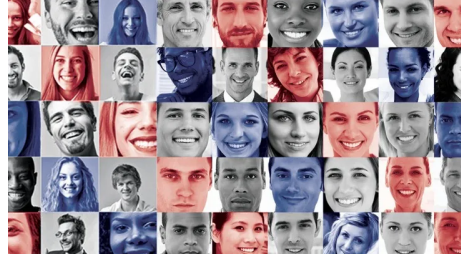
\includegraphics[width=\textwidth]{img/1.png}}
    \end{frame}
    \begin{frame}[plain]
        \center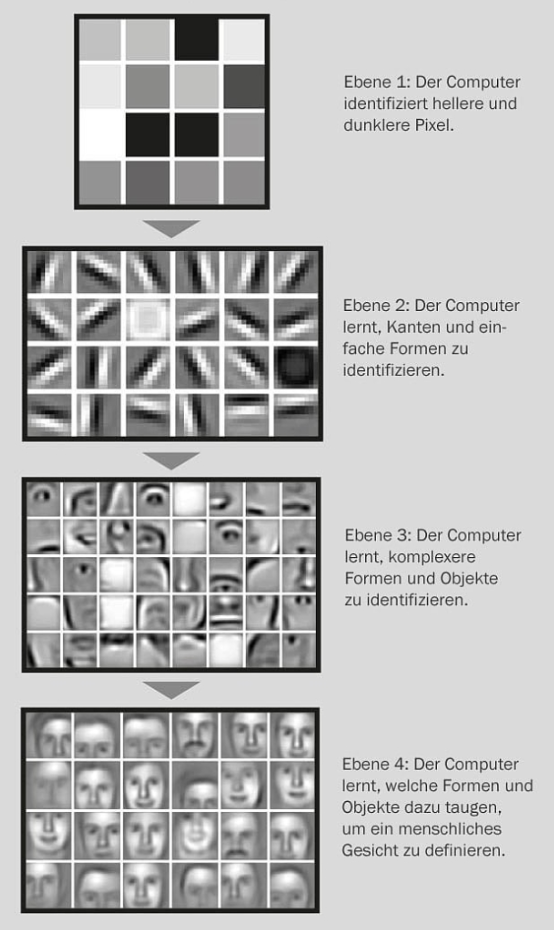
\includegraphics[height=\textheight]{img/4.png}
    \end{frame}
    \begin{frame} {One Neutron}
        \center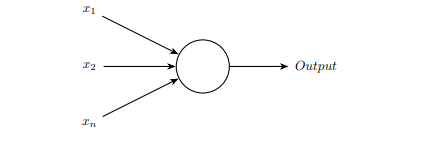
\includegraphics[width=\textwidth]{img/2.png}
    \end{frame}
    \begin{frame} {Neural Network}
        \center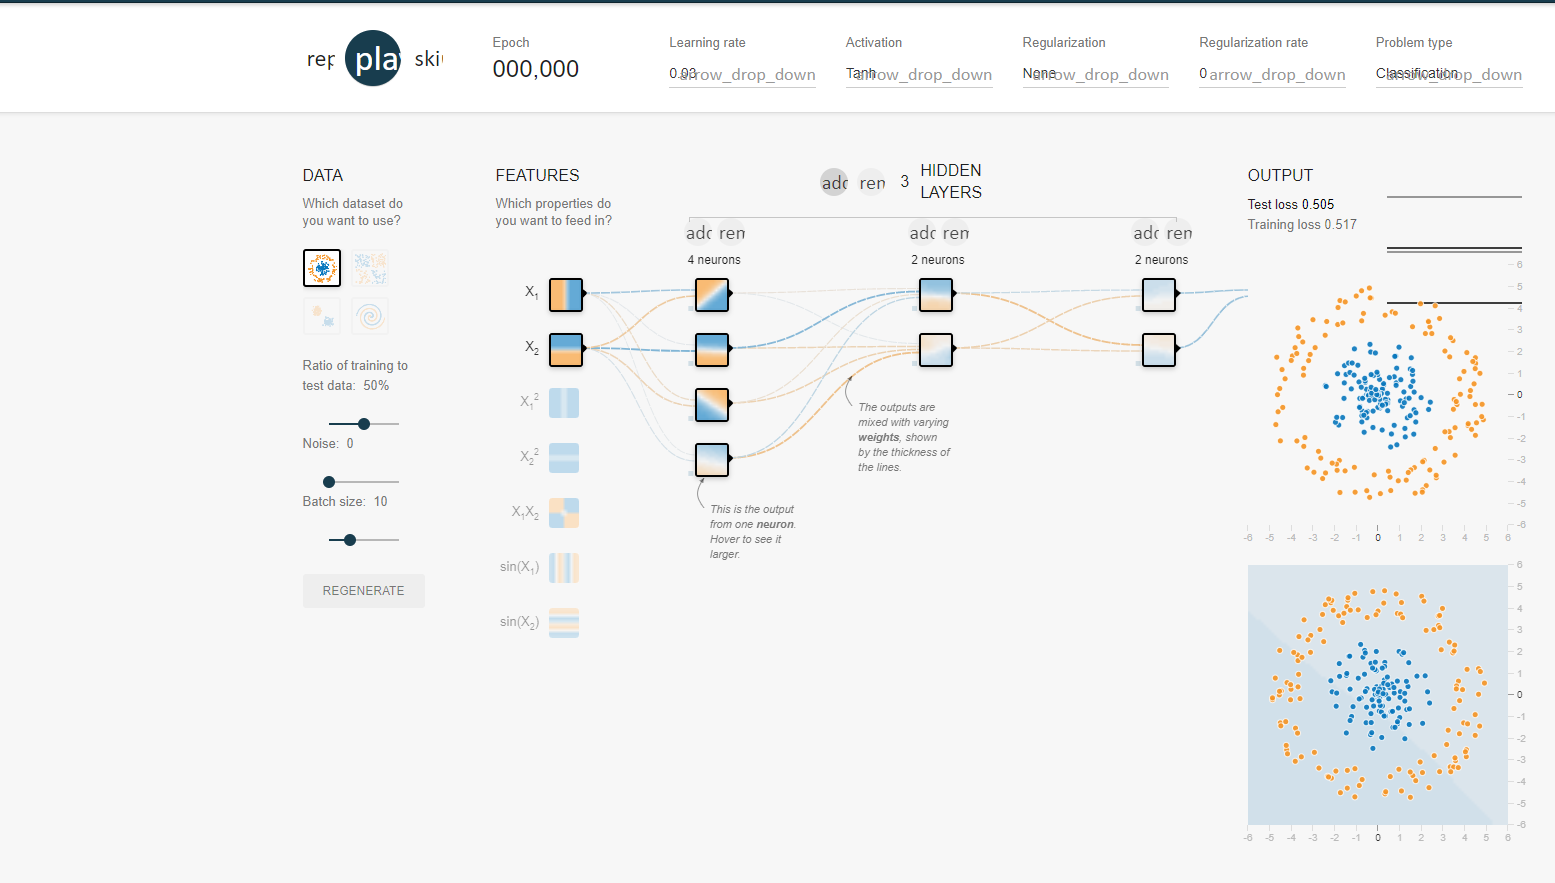
\includegraphics[width=\textwidth]{img/3.png}
    \end{frame}
    \begin{frame} {Deep Learning}
        \center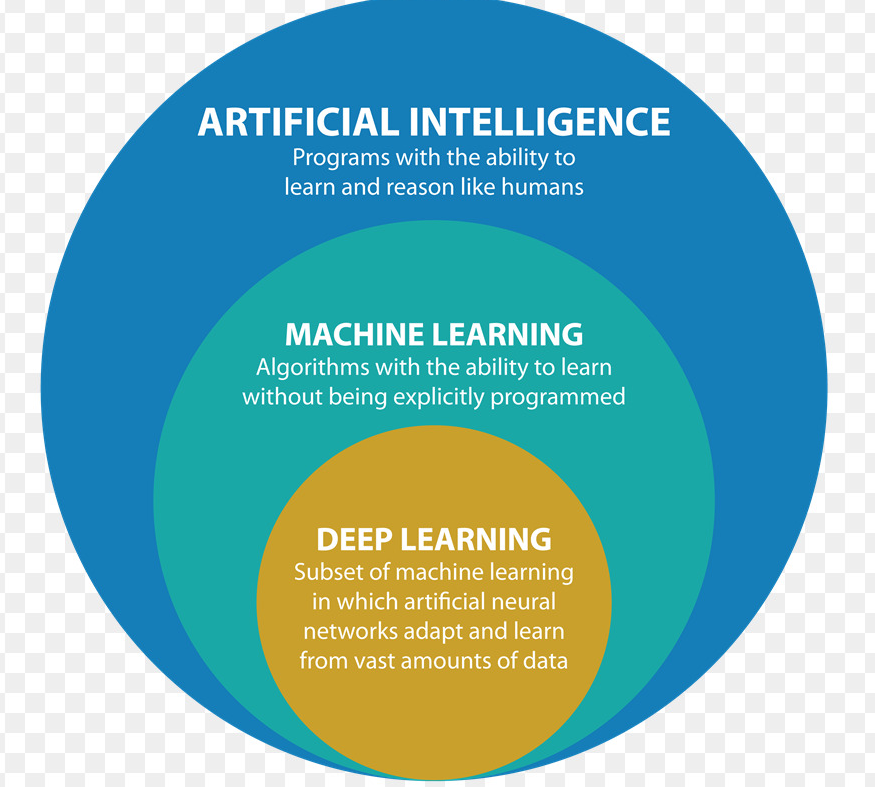
\includegraphics[width=\textwidth]{img/6.png}
    \end{frame}
        \begin{frame} {Image Recognition}
        \begin{itemize}[<+->]
           \item Classification
           \item Object recognition
           \item Instance segmentation
        \end{itemize}
        \begin{center}
            \action<+->{
                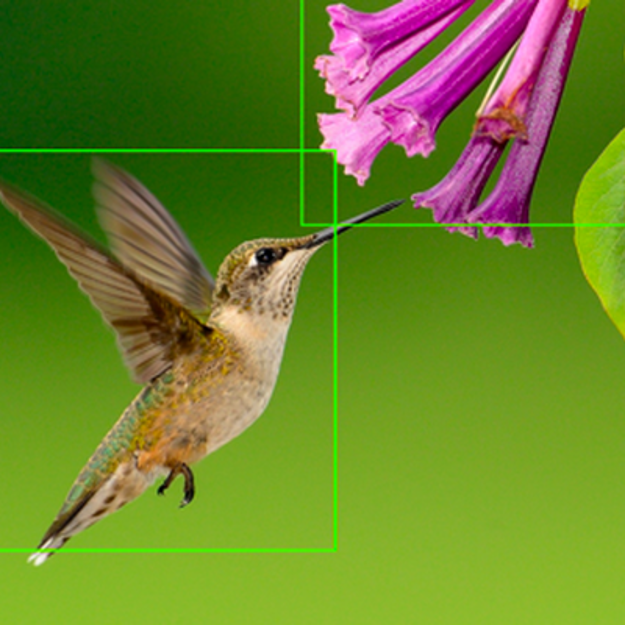
\includegraphics[width=.45\textwidth]{img/bird1.png}
                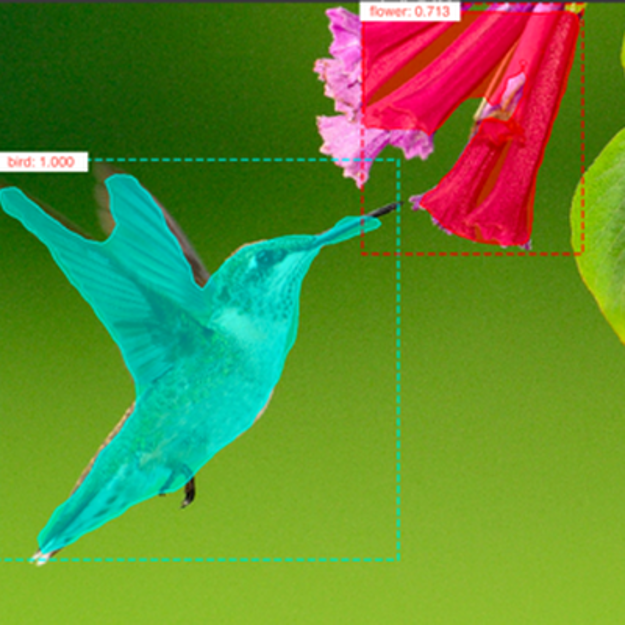
\includegraphics[width=.45\textwidth]{img/bird2.png}
            }
        \end{center}
    \end{frame}
    \begin{frame}[plain]
        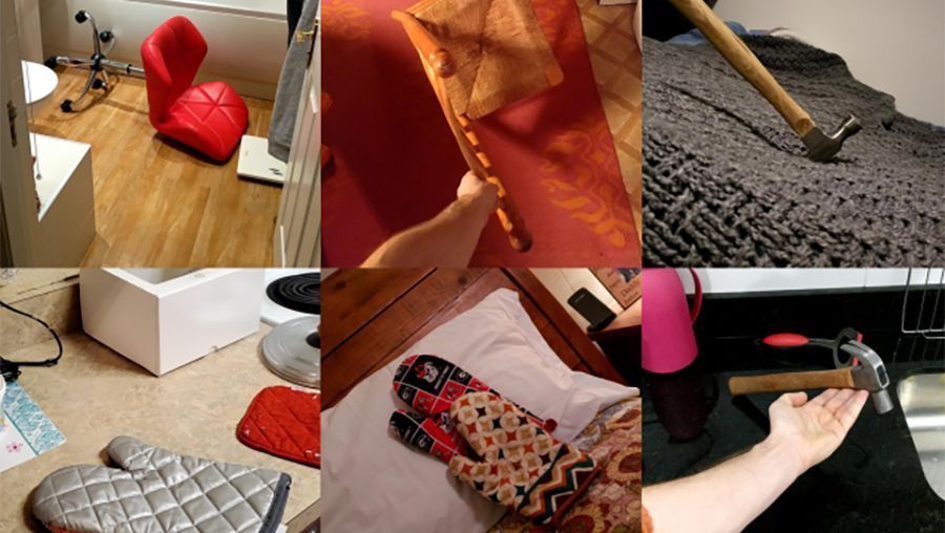
\includegraphics[width=\textwidth]{img/chaos.png}
    \end{frame}
    \begin{frame} {YOLO Algorithm}
        \center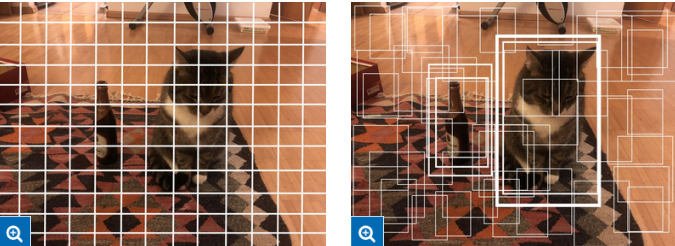
\includegraphics[width=\textwidth]{img/5.png}
    \end{frame}
    \begin{frame} {Data Processing with GDPR}
        \begin{itemize}[<+->]
           \item Big data needed, problem with GDPR
           \item Research projects need to stop or cant even start
           \item Solution $\rightarrow$ Federated Learning
        \end{itemize}        
    \end{frame}
% Sabine
    \begin{frame} {CIFAR-10}
        \begin{itemize}
            \item<+-> CIFAR-10 dataset (Canadian Institute For Advanced Research)
            \item<+-> Collection of images
            \item<+-> Contains 60.000 images
            \item<+-> 10 different classes: 
                \begin{enumerate}
                    \item airplanes,
                    \item cars,
                    \item birds,
                    \item cats,
                    \item deer,
                    \item dogs,
                    \item frogs,
                    \item horses,
                    \item ships,
                    \item trucks.
                \end{enumerate}
            \item<+-> 6.000 images per class
            \item<+-> Size 32 x 32
        \end{itemize}
    \end{frame}
\begin{frame} {Image Classification}
How does the image classification work?
\url{https://www.tensorflow.org/tutorials/images/cnn}

This tutorial demonstrates training a simple Convolutional Neural Network (CNN) to classify CIFAR images. (TensorFlow)
\end{frame}

\begin{frame} {SGD -- Stochastic gradient descent}
    \begin {itemize}[<+->]
        \item Iterative method for optimizing an objective function
        \item Replaces the actual gradient (calculated from the entire data set) by an estimate thereof (calculated from a randomly selected subset of the data)
        \item True gradient of $Q(w)$ is approximated by a gradient at a single example
        \item $w:=w - \eta \nabla Q_{i}(w)$
        \item Algorithm sweeps through the training set and performs the above update for each training example. Several passes can be made over the training set until the algorithm converges. If this is done, the data can be shuffled for each pass to prevent cycles
\end{itemize}
\end{frame}
\begin{frame} {SGD -- Possible pseudocode}
    \begin{center}
        \begin{minipage}[t]{.8\textwidth}
            \action<+->{choose an initial vector of parameters $w$ and learning rate $\eta$}\par
            \action<+->{\textbf{repeat} until an approximate minimum is obtained \textbf{do}}\par
            \action<+->{\hskip 2em randomly shuffle examples in the training set}\par
            \action<+->{\hskip 2em \textbf{for} $i = 1, 2, ..., n$ \textbf {do}}\par
            \action<+->{\hskip 4em $w:=w - \eta \nabla Q_{i}(w)$}
        \end{minipage}
        \end{center}
        
        \action<+->{source: Bottou, L\'eon (1998). "Online Algorithms and Stochastic Approximations". Online Learning and Neural Networks. Cambridge University Press. ISBN 978-0-521-65263-6.}
\end{frame}

\begin{frame} {Federated Learning}
        \begin{itemize}[<+->]
           \item Calculations on end device
           \item Results of calculations will be sent to global model
           \item Data privacy
        \end{itemize}        
       \action<+->{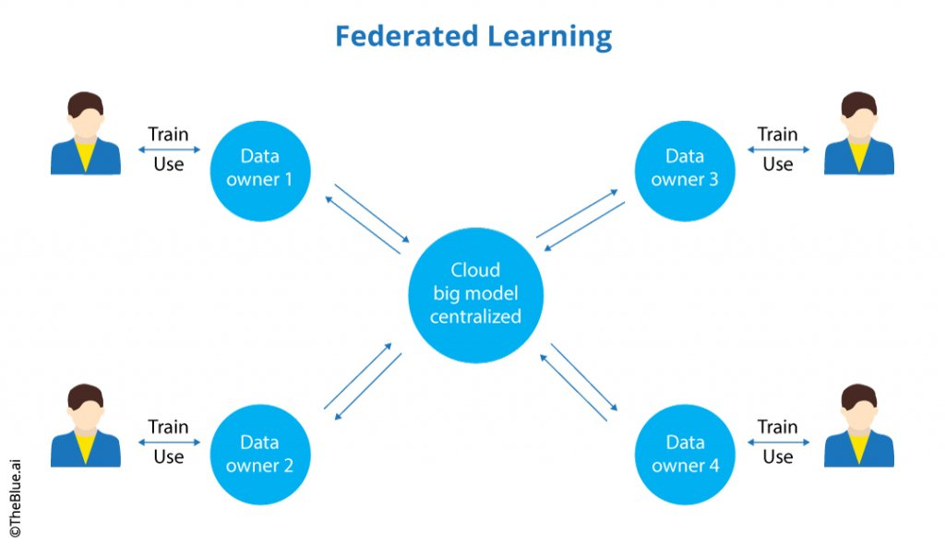
\includegraphics[width=\textwidth]{img/federated-learning.png}}
    \end{frame}

\begin{frame} {Federated Learning for image classification}
    \begin {itemize}[<+->]
        \item Can be simulated at TensorFlow:
        \url{https://www.tensorflow.org/federated/tutorials/federated_learning_for_image_classification}
        \item this simulation example uses the NIST (National Institute of Standards and Technology) dataset
    \end{itemize}
\end{frame}

\begin{frame} {NIST Handprinted Forms and Characters Database}
    \begin{itemize}[<+->]
        \item 3600 writers
        \item 810,000 character images
    \end{itemize}
    \action<+->{\center\includegraphics[width=\textwidth]{img/NIST.jpg}}
\end{frame}

\begin{frame} {Short overview Simulation results}
    \action<+->{Run a few rounds with a subset of the simulation data as not all users are always online}
    \action<+->{\begin{center}\includegraphics[width=\textwidth]{img/fedresult.jpg}\end{center}}\par
    \action<+->{Training loss is decreasing after each round of federated training, indicating the model is converging}\par
    \action<+->{The average metrics over all batches of data trained across all clients in the round}
\end{frame}
    \begin{frame} {Example Uses of Federated Learning}
        \begin{itemize}[<+->]
            \item Medicine
            \item Touch keyboard input prediction
            \vspace{1.5em}
            \item With learning based on user interactions labels are directly available
        \end{itemize}
    \end{frame}
    \begin{frame} {Practical Issues With Federated Learning}
        \begin{itemize}[<+->]
            \item Datasets are not representative of population
            \item Data differs from traditional centralized sources
            \item Users' usage styles differ greatly
            \item Many clients each with small datasets
            \item Mobile devices are often offline or on a slow or expensive connection
            \item Time zone differences
        \end{itemize}
    \end{frame}
    \begin{frame} {Resource Utilization}
        \begin{itemize}[<+->]
            \item Data center: Computational costs dominate
            \item Federated Learning: Communication costs dominate
            \item Computation essentially free
            \item Number of updates is minimized:
            \begin{itemize}
                \item by running on more clients in parallel (diminishing returns), or
                \item by performing more computations between updates.
            \end{itemize}
        \end{itemize}
    \end{frame}
    \begin{frame} {\texttt{FederatedAveraging} Algorithm}
        \begin{center}
                \begin{minipage}[t]{.8\textwidth}\small{
                \action<+->{\emph{Server}\par
                \textbf{Main}() \textbf{do}\par
                \hskip 2em initialize $w_0$\par
                \hskip 2em \textbf{for each} round $t = 1, 2, ...$ \textbf{do}\par
                    \hskip 4em $S_t \leftarrow$ random fraction of clients\par
                    \hskip 4em \textbf{for each} client $k \in S_t$ \textbf{in parallel do}\par
                        \hskip 6em $(w_{t+1}^k, n^k) \leftarrow$ ClientUpdate($k, w_t$)\par}
                    \action<3->{\hskip 4em $n \leftarrow n_1 + n_2 + ... + n_k$\par
                    \hskip 4em $w_{t+1} \leftarrow \sum_{k=1}^K \frac{n_k}{n} w_{t+1}^k$}

                        \action<+->{\vskip 1em \emph{Client $k$}\par
                        \textbf{ClientUpdate}($k$, $w$) \textbf{do}\par
                    \hskip 2em \textbf{for each} epoch from 1 to $n_k$ \textbf{do}\par
                        \hskip 4em $w \leftarrow w - \eta \nabla Q_{i}(w)$\par
                    \hskip 2em \textbf{return} $(w, n^k)$ to server}
                }\end{minipage}
        \end{center}
        \action<4->{\small{source: H. Brendan McMahan, et. al. (2016). "Communication-Efficient Learning of Deep Networks from Decentralized Data". arXiv.org.}}
    \end{frame}
    \begin{frame}[plain]
        \center{\Huge{The End}}
    \end{frame}
\end{document}
